\documentclass[tikz,convert={outfile=\jobname.svg}]{standalone}
\usepackage{xfrac}
\usetikzlibrary{arrows}
\begin{document}
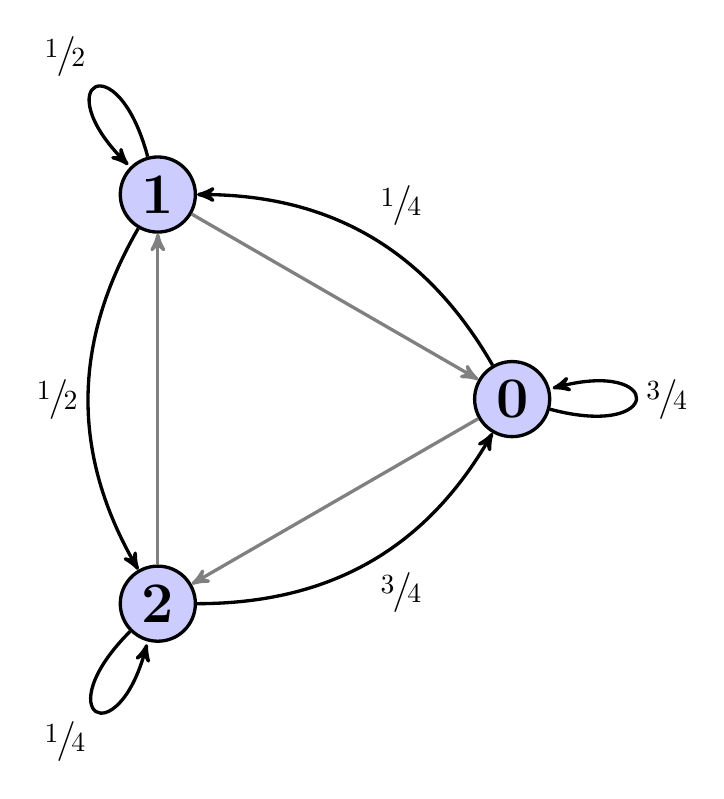
\begin{tikzpicture}[
  ->, >=stealth',
  scale=3,
  very thick,
  font=\Large,
  state/.style={circle,draw,fill=blue!20,font=\huge\bfseries}]

  \node (0) at (0:1)   [state] {0};
  \node (1) at (120:1) [state] {1};
  \node (2) at (240:1) [state] {2};

  \path
    (0) edge [out=-15,in=15,loop] node [right] {$\sfrac{3}{4}$} (0)
        edge [bend right] node [above right] {$\sfrac{1}{4}$} (1)
    (1) edge [out=105,in=135,loop] node [above left] {$\sfrac{1}{2}$} (1)
        edge [bend right] node [left] {$\sfrac{1}{2}$} (2)
    (2) edge [out=225,in=255,loop] node [below left] {$\sfrac{1}{4}$} (2)
        edge [bend right] node [below right] {$\sfrac{3}{4}$} (0);

  \path [gray]
    (2) edge (1)
    (1) edge (0)
    (0) edge (2);

\end{tikzpicture}
\end{document}
